
%[TODO: split approach from implementation]

\chapter[]{Modularisation des systèmes distribués}
%%% - Programme/Processus
%%% - Exécutable

Les programmes modernes ont une structure \textit{modulaire},
c'est-à-dire que leur code se décompose logiquement en différentes
parties relativement indépendantes, les \textit{modules}.  Cette
structure a de nombreux avantages, entre autres sur les plans du
développement, la maintenance et le déploiement des programmes.  Ce
mémoire porte sur la modularité dans le contexte des systèmes
distribués où le calcul est réparti sur de multiples ordinateurs
reliés en réseau.  Ce contexte pose des défis particuliers de
déploiement.

\section{Déploiement}

Le \textit{déploiement} d'un programme c'est sa mise en service pour
qu'il soit utilisable.  Ça consiste à installer une forme exécutable
du programme sur le(s) ordinateur(s) de sorte à pouvoir l'exécuter.
La façon de diffuser les modules, les stocker sur disque, les charger
en mémoire, etc. peut prendre plusieurs formes.

Un programme sous forme \textit{monolithique} contient dans son code exécutable
toutes les instructions exécutées par l'ordinateur.  Cette forme était la norme
dans les premiers systèmes informatiques, et l'est toujours pour les systèmes
embarqués qui n'ont pas de système d'exploitation indépendant.  Lorsqu'un
système d'exploitation est disponible sur l'ordinateur on peut le considérer
comme étant un module puisqu'il offre des services précis avec une interface
standardisée.  Dans ce cas, un programme peut prendre la forme d'un seul
fichier de code qui, à son exécution, communiquera avec le système
d'exploitation pour accéder à ses services.  Ce genre de fichier exécutable est
obtenu par une \textit{édition de liens statique} qui combine en un seul
fichier tous les modules (à l'exception du système d'exploitation).  Par
rapport à la forme monolithique, cette organisation simplifie le développement,
car le programmeur n'a pas à se soucier du développement des services de base
comme l'accès aux fichiers, la gestion des processus et de la mémoire, etc.  Le
programme peut être diffusé à d'autres ordinateurs ayant le même système
d'exploitation simplement en y transférant le fichier exécutable.

L'édition de lien statique a un certain nombre de défauts. L'état des
modules utilisés au moment de l'édition de liens est figé au sein du
programme, ce qui empêche la mise à jour individuelle des modules à de nouvelles versions. Il faut
recompiler tous les modules qui ont subi une mise à jour et refaire l'édition de liens du
programme principal. Le coût en temps et l'effort pour un petit changement
sont importants.  Le chapitre \ref{ch:loading-model} va détailler plus en profondeur
ces problèmes.

% Le même module est chargé plus d'une fois.
L'édition de liens peut se faire paresseusement par le système d'exploitation à
l'exécution du programme, ce qu'on appelle l'\textit{édition de liens
dynamiques}.  Cela permet de garder la structure modulaire au
\textit{déploiement}.  Chaque module est une composante séparée du programme
principal.  Ces modules sont lus du disque et chargés en mémoire durant
l'exécution du programme.  Ce chargement est effectué par l'\textit{éditeur de
liens dynamique du système d'exploitation}~\cite{DBLP:journals/cse/BeazleyWC01,DBLP:journals/spe/HoO91}
qui s'occupe de lier les fonctionnalités des modules au programme principal.
% Le chapitre % chapter or section \ref{ch:module_systems} explique plus en
% profondeur le fonctionnement de l'éditeur de liens dynamique du système
% d'exploitation.
L'avantage principal du chargement dynamique de module est la
possibilité de mise à jour individuelle d'un module sans avoir à lier le
programme principal; dans le modèle statique, le programme principal doit être
lié à nouveau avec les modules.  Les modules chargés dynamiquement par le
système d'exploitation peuvent être partagés entre différents programmes.
% Ce type de module, les \textit{bibliothèques partagées}, est décrit dans le
% chapitre \ref{ch:module_systems}.

% % Migration de code dans un système distribué.
% - Transmission de tâche entre des machines d'un système distribué.
%   - Un module absent sur la machine distante nécessaire à l'exécution
%   de la tâche transmise.
%     - Télécharger le module d'un serveur dédié.
%     - Revient au chargement dynamique de ce module.
\section{Systèmes distribués}

Un \textit{système distribué} est un groupe d'ordinateurs, les
\textit{nœuds} de calcul, reliés en réseau afin qu'ils puissent
échanger des messages et coordonner leurs activités.  Chaque nœud peut
exécuter le même code que les autres nœuds ou bien un code spécialisé
au rôle qu'il joue au sein du système (e.g.~serveur vs ~client).
D'une façon ou de l'autre on parlera de l'ensemble du code comme étant
le \textit{programme distribué} qu'ils exécutent.

Les programmes distribués posent de nouveaux problèmes de déploiement,
car les nœuds sont rarement identiques.  Ils peuvent avoir des
architectures matérielles différentes, et/ou des ressources et
périphériques différents, et/ou des systèmes d'exploitation
différents.  Il est à noter que ces caractéristiques peuvent changer
pendant la période d'exploitation du programme, par exemple lors de
mise à jour du matériel et du système d'exploitation.  Ce problème est
exacerbé par le \textit{code mobile}, c'est-à-dire un calcul en
exécution sur un nœud qui se déplace, ou \textit{migre}, sur un autre
nœud pour poursuivre son exécution.  Cette \textit{migration de
  tâche} est utile pour améliorer la performance lorsque le nœud
destinataire est plus puissant ou possède localement les données
utilisées par la tâche migrée.  Finalement, dans le cas de programmes
distribués offrant un service à l'externe, on veut minimiser les
interruptions de service causées par les mises à jour du système ou
d'une de ses parties, que ce soit 1) au niveau matériel et/ou le
système d'exploitation ou 2) le programme distribué lui-même.  Dans le
premier cas, la migration de tâche peut être utilisée pour migrer le
service à un autre nœud le temps que se fasse la mise à jour.  Dans
le deuxième cas, on aimerait utiliser les nouveaux modules
modifiés sans avoir à arrêter le programme et le redémarrer.

Il apparait donc avantageux que le code du programme distribué prenne
une forme exécutable \textit{portable} qui peut s'adapter aux
particularités de chaque nœud sans demander au développeur de
modifier ou recompiler le programme distribué.  Idéalement, cette
portabilité ne devrait pas causer des pertes de performance.  D'autre
part, la possibilité de substituer une version d'un module par une
nouvelle version sans interruption du programme est attrayante.

\section{Modules versionnés}
%
Nous définissons le terme \textit{version de module} comme étant tout
simplement un état de son code.  Ainsi, lorsqu'on fait une
modification au code d'un module pour corriger un problème ou pour
étendre ses fonctionnalités on obtient une nouvelle version du module.
La version d'un module est donc essentielle pour identifier son code,
et donc sa fonctionnalité, de façon précise. Pour permettre plusieurs
versions d'un module au sein d'un programme, il est important que
chaque version des modules soit distinguable.
Lors de la migration de code, il est possible que plusieurs versions
d'un module soient chargées pour accéder des fonctionnalités.

%[TODO: expliquer les ramification et que c'est une partie essentielle de ton
% système de module.]

Le concept de version de module n'est pas intégré à la sémantique de
plusieurs langages de programmation.  En Python et Java les
modules sont référés dans le code avec un nom qui n'inclut pas la
version.  Go est un exemple de langage de programmation qui
permet d'inclure la version lorsqu'on réfère à un module.

Dans les systèmes qui considèrent chaque version d'un module comme un
module différent, il devient possible d'écrire des programmes qui
utilisent de multiples versions d'un module simultanément. Cela peut
amener certains problèmes de conflit entre les versions. Ces conflits
peuvent être observés dans les langages interprétés comme JavaScript
ou dans les langages compilés comme C/C++. Les conflits peuvent être
dans les noms des fonctions du module ou dans des variables globales
partagées entre plusieurs versions du module.

% Nous reviendrons sur les modules versionnés au chapitre
% \ref{ch:module_systems}, car ce concept est essentiel dans
% notre approche de modularisation.

\section{Code mobile}

Dans un système distribué, il est utile d'amorcer des calculs sur un
nœud à partir d'un autre.
Cela peut se faire avec un appel RPC (\textit{Remote
Procedure Call}) ou par \textit{migration de tâches}.  Un appel RPC correspond
à une requête d'exécution d'un calcul sur un nœud distant. Une migration de
tâche copie l'état courant de la tâche et l'envoie sur le nœud distant où son
exécution est continuée.

Les appels RPC sont présents dans plusieurs systèmes et langages de
programmation.  Le protocole \texttt{ssh} permet une forme d'appel RPC par
invocation de processus sur un nœud distant. Java offre les appels distants par un
mécanisme similaire au RPC nommé RMI (\textit{Remote Method Invocation}).
Le langage C offre des bibliothèques qui implémentent un protocole de RPC.
Ces variantes de RPC sont limitées aux fonctionnalités fournies par le nœud distant.
Pour le bon fonctionnement de cette approche, il est nécessaire que le
service demandé soit déjà déployé sur la machine distante.

La migration de tâche permet de transférer une tâche d'un nœud à un autre.  Ce
mécanisme a été implémenté dans différents langages comme
Erlang~\cite{M_mobileintelligent}, Java~\cite{And98transparentmigration},
Scheme~\cite{Sumii00animplementation,DBLP:conf/erlang/Germain06},
 % \cite{TermiteScheme},
JavaScript~\cite{DEV2017transparentmigration}. Ce mécanisme requiert
typiquement que l'ensemble du code soit disponible sur le nœud distant.

Stefan Fünfrocken a conçu un système d'agents mobiles écrit en
Java~\cite{And98transparentmigration}. Il capture l'état présent du programme
qui inclut les valeurs et les types de toutes les variables de chaque objet.
La pile des appels de méthode avec les valeurs de toutes les variables est
aussi incluse dans l'état du programme.  Ces informations sont transmises au
nœud distant qui les utilise pour reconstruire le programme initial.
L'ensemble des méthodes sur le nœud de départ est présent sur le nœud
d'arrivée.

Le système implémenté dans le langage de programmation
Erlang~\cite{M_mobileintelligent} qui implémente des agents mobiles requiert
que le code soit disponible sur le nœud destination.

Le système de migration en JavaScript~\cite{DEV2017transparentmigration}
utilise des nœuds pour conserver le code. Il est basé sur le fait que le code
des agents est connu par les nœuds spécialisés. Puisque le code des agents est
connu, il suffit de transmettre l'état de l'agent pour effectuer une migration.
%Ce modèle JavaScript ressemble à celui implémenté dans Gambit lors de la
%transmission de procédures compilées par l'utilisation de nœuds pour conserver
%le code.
Le scénario de migration de code présenté dans le chapitre
\ref{ch:scheme_concepts} nous a inspiré dans la conception d'un système de
module.
Notre motivation est la migration de code entre des nœuds d'un système
distribué comme présenté à la fin du chapitre \ref{ch:scheme_concepts}.  Nous
avons développé un système de module pour le langage de programmation Scheme
qui offre la possibilité de migrer un agent sur un nœud qui ne connait pas à
priori le code de l'agent, et qui permet à des versions multiples d'un module
de coexister.

Notre point de vue est que la migration de code ne devrait pas
demander une préconfiguration des nœuds, car une gestion coordonnée de
tous les nœuds d'un système distribué est difficile ou impossible
lorsqu'il y a plusieurs nœuds et/ou des nœuds de nature différente
et/ou il n'y a pas un gestionnaire unique de l'ensemble des nœuds.
Même dans le cas où les nœuds sont sous le contrôle d'un unique
gestionnaire, il serait avantageux de ne pas interrompre le
fonctionnement du système distribué lorsque les modules sont
améliorés.

%\section{Approche de transmission}
%[TODO: approche]


%[TODO: contrib]
Les contributions de ce travail sont la conception d'un système de module pour
les systèmes distribués et son intégration dans Gambit Scheme. Ce système
permet la diffusion des modules compilés entre les nœuds d'un système
distribué sans préconfiguration des modules avec le code et permettant
de multiples versions d'un module de coexister.
% Nous avons conçu un système de module pour les systèmes distribués.  Nous
% l'avons intégré dans le système Gambit Scheme.

% \begin{itemize}
%   \item Modules mobiles.
%   \item Transmission de code compilé entre des machine de différente
%     architecture et système d'exploitation.
%   \item Mise à jour des programme sans interruption de service.
% \end{itemize}

\section{Survol}

Le chapitre \ref{ch:scheme_concepts} explique les approches existantes de
modularisation en Scheme.  Le chapitre \ref{ch:modules_implementation}
traite de l'implémentation du système de module et son intégration dans Gambit,
un compilateur/interprète performant pour Scheme. Le chapitre
\ref{ch:loading-model} explique les mécanismes de chargement des modules.  Le
chapitre \ref{ch:module_management} traite de l'organisation générale des
modules. Le chapitre \ref{ch:task_migration} traite de la diffusion des modules
et de la migration de tâche.  Le chapitre \ref{ch:evaluation} présente une
évaluation du système de modules avec des résultats d'expériences effectuées
entre des systèmes d'exploitation et architectures différentes.


% XXX: Agent TCL

% \section{Linkage statique}
% Cette forme d'édition de lien permet la création de binaire qui indépendant
% qui facilite le déploiement.

%\section{Linkage dynamique}

%--------------------------END---------------------------

% Un programme sur une des machine du système distribué qui se fait transmettre
% une tâche peut devoir exécuter une fonctionnalité d'un module absent
% localement. Cela nécessite un téléchargement du module contenant la
% fonctionnalité demandé d'un serveur dédié. Une fois le module installé, il faut
% le charger dynamiquement.

% ==> motiver (quels problèmes ça cause le link statique) et expliquer le chargement dynamique, système distribué, etc


%Problème du link statique\\
% - Gèle les versions des modules au sein du programme. \\
%    -> Comment la maintenance d'un programme lié statiquement? \\
%    - Le temps de compilation. (Coût d'un changement est important) \\
% - La taille du programme peut être plus importante.
% - Le même module est chargé plusieurs fois en mémoire.



% Dans les systèmes comme DOS, les programmes ou modules devaient contenir toutes les
% informations nécessaire pour s'exécuter. De tels programmes sont dit lié
% statiquement dans le sens qu'il ne dépende que de l'architecture sur laquelle il
% a été construit. La construction des modules requière deux étapes. La compilation
% de fichier source en fichier objet contenant le nom et le code des fonction.
% L'édition des liens qui réunit un plusieurs fichiers objets en un module.
% Dans le cas d'un seul fichier l'édition des liens ne fait que transformer le fichier
% objet en fichier exécutable.

% \begin{figure}[ht]
%   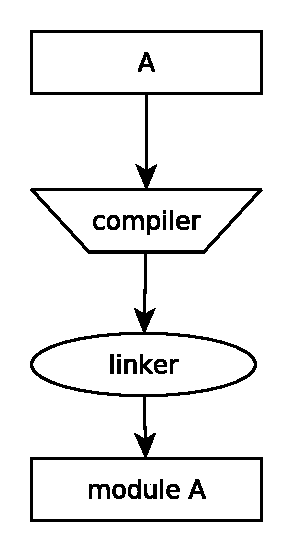
\includegraphics[width=0.20\linewidth]{figures/basic_module_compilation.pdf}
%   \caption{Construction du module A à partir des sources.}
% \end{figure}

%La création d'exécutable inclut deux étapes importantes, la compilation et
%l'édition des liens. La première étape consiste à prendre un fichier de code
%source et de le traduire en fichier objet, que l'on retrouve souvent avec
%l'extension \verb|.o| ou \verb|.obj|, qui contient la représentation des
%procédures compréhensible par le processeur. Ces fichiers objets ne sont pas
%encore exécutable pour autant, il faut tout d'abord effectuer la seconde étape,
%qui va les regrouper en un exécutable. Le programme qui s'occupe de l'édition
%des liens est le \textit{linker}, la version GNU se nomme \verb|ld|.  Voici
%l'exemple de la création d'un exécutable composé des fichiers sources C
%\verb|main.c| et \verb|foo.c|:
%
%\begin{figure}[ht]
%    \begin{minipage}[t]{0.5\textwidth}
%\begin{verbatim}
%# Compilation
%gcc -c main.c -o main.o
%gcc -c foo.c -o foo.o
%# Édition de liens
%ld -o main.exe main.o foo.o
%\end{verbatim}
%    \end{minipage}
%
%    \caption{Exemple de création d'un exécutable}
%\end{figure}



%Cela implique que ils possible de retrouvé une dépendance en diamant tel que représenter
%dans la figure-\ref{fig:dep1} qui peut causer un problème. % Détailler
%\begin{figure}[ht] %% Pas juste valide pour scheme.
%  \begin{center}
%    %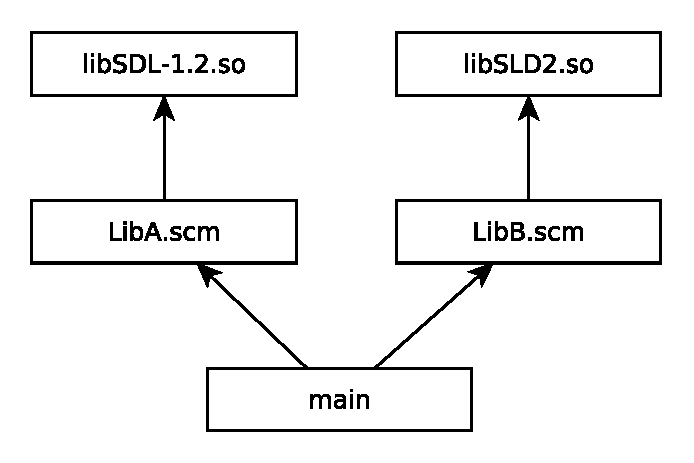
\includegraphics[width=4cm]{figures/SchemeLibrary}
%    \caption{Dépendence en diamant}
%    \label{fig:dep1}
%  \end{center}
%\end{figure}

%% NOTE: Soit P un processus, execution(A, P=[A,B]) == execution(A, P=[A]).
%Soit un processus \textbf{P} qui réfère aux bibliothèques \textbf{A} et \textbf{B}.
%Une bibliothèque peut masquer les symboles d'une autre bibliothèque chargé dans le même processus.
%La bibliothèque \textbf{A} coexiste avec la bibliothèque \textbf{B} si la \textbf{A}
%ne masque pas des symboles ne \textbf{B} qui amène un comportement non défini.


% Historiquement, il y avait un problème avec la coexistence entre deux dll sous Window. TODO: devellopper

% - Système distribué (Actor), non limité par la diversité des bibliothèque.


% TODO:
%La coexistance entre plusieurs versions d'une même bibliothèque
%===========================================================
%
% - Définition d'une bibliothèque
%   - Nom symboles:
%     - Fonction
%     - Variables global
%     - Structure de donnée
%     - Macro (Compilation)
%
%- Définition par coexistence de plusieurs bibliothèque.
%- Pourquoi est-ce utile?
%- Conditions nécessaire pour la coexistence entre plusieurs versions d'une même bibliothèque soit possible.
%  - Data race.
%  - État partagé.
%- Système d'exploitation (DOS)


